
%!TEX root = ../thesis.tex
%*******************************************************************************
%****************************** Third Chapter **********************************
%*******************************************************************************
\chapter{Calibration}

% **************************** Define Graphics Path **************************
\ifpdf
    \graphicspath{{Chapter7/Figs/Raster/}{Chapter7/Figs/PDF/}{Chapter7/Figs/}}
\else
    \graphicspath{{Chapter7/Figs/Vector/}{Chapter7/Figs/}}
\fi

%********************************** %Opening  **************************************

Chapter 7 Opening

\newpage
%********************************** %First Section  **************************************

\section{Electron Lifetime}

\subsection{Measurement Procedure}

\subsection{Lifetime Correction}

\subsection{Bias Study From Diffusion and Space Charge Effects}

\subsection{Look Up Curve}

\subsection{Bias Study From Geometry of Cosmic Ray Tracks}

\subsection{Concluding Remarks}
%********************************** %First Section  **************************************

\section{Delta Ray Fluctuations on Recombination Simulation}

%Introduce why this is important
%TODO: Mention ICARUS paper
As discussed in Chapter \ref{Chapter6}, simulation plays a vital role in neutrino physics.
The need to correctly simulate physics processes must be addressed in order to validate against data and build towards a data-driven simulation.
The physics process of this simulated study is recombination, which drives the charge and light yield.
As described in Sec. \ref{sec:recomb}, the recombination model employed at SBND is an phenomenological model, with parameters that have been experimentally measured by ArgoNeuT and tuned for simulation to match data \cite{argoneut_recomb}.
The Modified Box (ModBox) model approximates the recombination probability based on a cylindrical column surrounding a track-like charge deposition.
This volume treatment effectively accounts for microphysics processes produced along the track, such as delta rays, as some additional charges of the track itself.
This approximation has proven to work well for the MeV to GeV-scale interactions, energy range relevant to LArTPC detector, however, breaks down when applying to keV-scale interactions.
The NEST collaboration has pointed out non-linear fluctuations in recombination at increasingly smaller scales, which is currently not well-described by the ModBox model \cite{NEST}. 
Moreover, the ArgoNeuT collaboration has also proposed that microphysics effects could lead to disagreements in recombination theory and simulation and measurement \cite{argoneut_recomb}.

One microphysics process that can affect recombination, highlighted by both NEST and ArgoNeuT collaborations, is delta ray.
Delta rays are high $dE/dx$ knock-out electrons with energy as low as 1 keV.
As shown in Fig. \ref{fig:delta_ray_evd}, delta rays can be seen as short tracks produced along a longer primary track, in this case, a cosmic muon.
Since delta rays have high $dE/dx$, they are associated with a smaller recombination factor, producing more scintillation photons  while quenching ionisation electrons.
This simulation investigation examines how fluctuation in delta rays impacts the recombination simulation, and consequently, the energy-charge scales of different particle types.
Sec. \ref{sec:simDeltaRay} explains the simulation framework of delta rays and recombination, an expresses some concerns associated with the current simulation framework.
Sec. \ref{sec:impactDeltaRay} and \ref{sec:impactStepLimit} describes the impacts of varying configurable simulation handles associated with delta rays on particle calorimetry.
Finally, Sec. \ref{sec:concludeDeltaRay} suggest recommendations for future work, with a focus on data-driven approaches.

\begin{figure}[thp] 
\centering    
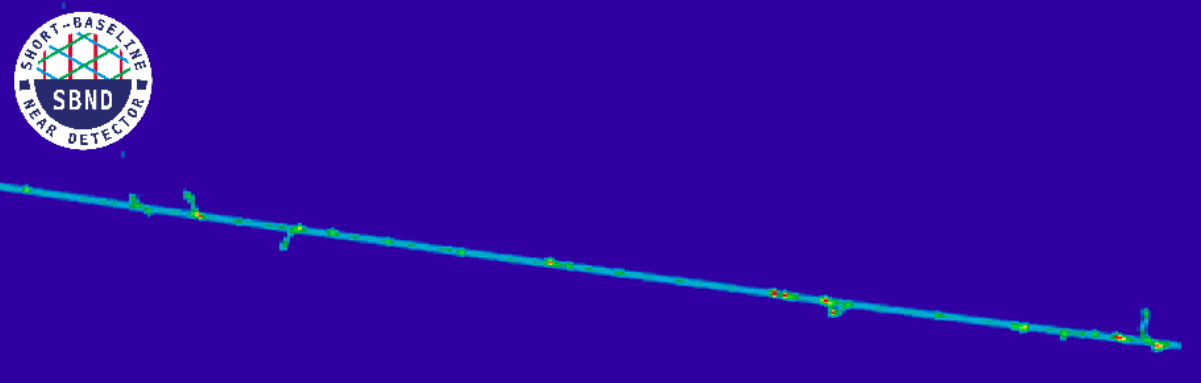
\includegraphics[width=0.85\textwidth]{delta_ray_evd}
\caption[delta_ray_evd]{
Event display of a segment a simulated cosmic muon track, with many little delta rays produced along the primary track.
}
\label{fig:delta_ray_evd}
\end{figure}

\subsection{Simulation of Delta Rays and Recombination}
\label{sec:simDeltaRay}
%TODO: Geant4 or LArG4?
%Describe delta rays simulation
The physics of particle propagation from creation to detection point is simulated at the Geant4 stage as described in Chapter \ref{}.
This stage is responsible to propagate the primary particle step by step and apply physics processes to each step $dx$.
Geant4 simulates the physics of energy loss due to ionisation $dE$ as two intertwined processes: (1) a continuous energy loss of the primary particle along a step and (2) a discrete energy loss at the end of a step to produce delta rays.
The distribution of energy deposition per step $dE/dx$ for each process is defined by an energy threshold.
For the continuous energy loss process, the energy threshold restricts the upper limit of the stopping power so that the mean energy loss is less than the threshold.
For the delta ray production process, the energy threshold defines the lower limit of the kinetic energy of the generated delta rays.
In other words, the energy threshold determines how much energy deposition is shared between the primary particle and the delta rays. 
The lower the threshold, the more energy deposition is carried away by the delta rays instead of the primary particle. 

In Geant4 terminology, this energy threshold is also known as the secondary production threshold, where the minimum kinetic energy requirement for delta ray production is defined as the minimum distance the generated delta ray must be able to traverse in a given material. 
For the standard simulation in SBND, the secondary production threshold for delta rays in a LAr medium is set as 700 $\mu$m, equivalent to delta ray having a kinetic energy of 273 keV.
Moreover, the maximum length $dx$ that the particle can propagate per step is set as 0.3 mm.
This setup allows for a more feasible computation by not generating and tracking all possible low energy delta rays.

%Describe ionandscint module
Recombination is simulated for each energy deposition step to determine the charge and light yield.
The recombination factor $R$ is first calculated taking inputs of $dE/dx$ of the step and the electric field of the detector at the position of the step.
The numbers of ionisation electrons and scintillation photons are then calculated according to Eq. \ref{} and \ref{}.

%potential issue
As discussed previously, the ModBox model for calculating the recombination factor $R$ uses parameters measured by ArgoneuT \cite{}, that employed a stopping proton sample with a wire pitch of 3 mm.
Thus, the simulation of delta rays and recombination can give rise to several concerns.
The first concern is the assumption of a \textit{universal} recombination factor $R$, where the same value is applied to different types of ionising particle which can influence the local ionisation density differently. 
Secondly, the second production threshold on delta rays remove low energy ionisation electrons, which are produced in reality and can fluctuate the local recombination factor. 
The last concern is the step length $dx$ configured to be one order of magnitude smaller than the wire pitch of both ArgoneuT and SBND, resulting in the effective recombination $R$ being applied at a microscopic scale.

%how to validate
The simulation investigation was set up to address individual concern as well as to better understand their impacts on recombination.
A truth calorimetry comparison was carried out on two identical samples of muons and protons. 
The particles were generated with a fixed energy of 1 GeV, uniform in positional and angular distributions.
The Geant4 stage was configured such that the particle can only deposit energy via ionisation.
The first study is presented in Sec. \ref{}, focusing on the fluctuations in delta ray by lowering the secondary production threshold, allowing for more low energy delta rays to be produced.
The second study is presented in Sec. \ref{}, with the step length $dx$ configured to be the same as SBND wire pitch. 

\subsection{Impacts of Delta Ray Fluctuations}
\label{sec:impactDeltaRay}

Fluctuations in delta rays were examined at different values of the secondary production thresholds ranging from 700 $\mu$m to 1 $\mu$m.
This is equivalent to generating delta rays of minimum kinetic energy ranging from 273 keV to as low as 1 keV.
The charge-to-energy estimation was calculated using the ModBox recombination model with the ArgoneuT parameters as follow

\begin{equation}
	dE/dx = \left(\exp{\left(\beta W_{ion} \cdot dQ/dx \right)} -\alpha \right)/\beta
\end{equation}
where $\alpha = 0.93$ and $\beta = 0.30$ cm/MeV. 
This recombination model for an electric field of 500 V/cm is plotted in Fig. \ref{} of Chapter \ref{}.

The calorimetry plots of $dQ/dx$ to $dE/dx$ for proton are shown in Fig. \ref{} and Fig. \ref{}, for the secondary production threshold at 700 $\mu$m and 1 $\mu$m respectively.
The calorimetry is plotted for the proton residual range from 1 cm to 90 cm, which covers the full track length. 
The proton $dE/dx$ proton ranges from 2 MeV/cm to 18 MeV/cm, allowing for the examination of delta ray fluctuation impacts at both low and high spectrum of $dE/dx$. 
For the secondary production threshold of 700 um, the calorimetry distribution precisely follows the ModBox model with the ArgoNeuT parameters.
The good agreement is expected since the standard simulation of SBND is similar to the described simulation framework by ArgoNeuT \ref{}: (1) the maximum step length $dx$ was restricted to be 0.3 mm and (2) the energy loss due to delta rays was not included in recombination.

However for the secondary production threshold of 1 um, deviations away from the ModBox model occurs, such that the energy-charge scale shifts in opposite directions at low $dE/dx$ compared to high $dE/dx$. 
Lowering the secondary production threshold leads to more energy deposition carried by the delta rays instead of the proton, and thus, delta rays have greater influence on recombination.
At the low $dE/dx$ spectrum of proton, delta rays have higher $dE/dx$ than that of proton, resulting in the effective recombination factor being quenched. 
The opposite effect is seen at the high $dE/dx$ spectrum of proton, resulting in the effective recombination factor increases.
 
In order to compare $dQ/dx$ quantitatively at the same $dE/dx$ bin, the mean $dQ/dx$ is calculated per bin.
%This then allows the determination of the output simulated recombination factor, given as $dE/dx / (W \times dQ/dx)$.
The resulting plots is shown in Fig. \ref{} for the secondary production thresholds at 700, 10, 5, 1 $\mu$m, equivalent to delta rays with minimum kinetic energy of 272.58, 14.60, 2.58, 1.06 and 0.99 keV.
In order to examine the magnitude of impacts from delta rays fluctuations on the energy-charge scale, the percentage difference of the mean $dQ/dx$ relative to the ModBox model are plotted in Fig. \ref{}.
Lowering the kinetic energy of delta rays results in two key trends.
Firstly, the $dE/dx$ position at which the proton energy-charge scale shifts in opposite directions, increases with lower delta ray kinetic energy. 
Secondly, the magnitude of the deviations is also dependent on the delta ray kinetic energy. 
At low $dE/dx$, the magnitude of the effective recombination quenching is the greatest for the secondary production threshold set as 1 $\mu$m. 
Meanwhile at high $dE/dx$, the effective recombination is the highest for the secondary threshold set as 10 $\mu$m. 
This is evident that delta ray fluctuations determine how much the proton is \textit{dressed} in delta rays, and can greatly influence the effective recombination factor across the $dE/dx$ spectrum of proton. 

The calorimetry plot for muon is plotted in Fig. \ref{}, for the secondary production threshold at 700 $\mu$m and 1 $\mu$m respectively.
No restriction on the muon residual range is applied, to fully cover the track length from 1 to 400 cm.
Two distinct distributions can be seen, one linear prong from the MIP muon region, and another one that follows curve of the ModBox model indicating the muon stopping region. 
%The linear distribution is due to the dressing the primary muon with very high energy delta rays, which have a linear energy-charge scale. 
%This result in this linear feature that has been well observed experimentally with MIP muons. 
The linear energy-charge scale has been well-observed experimentally with MIP muons \cite{}.
In order to examine the stopping region exclusively, a residual range requirement of less than 10 cm is applied, as shown Fig. \ref{} and Fig. \ref{}. 
Some remnants of the MIP muon distribution can still be seen in the $dE/dx$ range between 4 to 12 MeV/cm. 
Similarly to proton at the low $dE/dx$ scale, delta rays with lower kinetic energy results in quenching the effective recombination factor. 
The mean $dQ/dx$ of muon and its percentage difference relative to the ModBox model are also plotted as shown in Fig. \ref{}.
The same behaviour as proton is observed such that the magnitude of the effective recombination quenching increases with lower delta ray kinetic energy.
Nonetheless, the magnitude of the quenching is larger for muon compared to proton.
The difference is driven by how each particle type is \textit{dressed} in a different amount delta rays even at the same simulation configuration for delta rays.

The effects of delta rays on recombination also extends to smearing of the energy-charge scale.
In order to de-tangle how the Geant4 simulation framework handles the smearing due delta rays, additional study was carried by isolating only the energy deposition of the primary particle.
Fig. \ref{} shows the $dE/dx$ of the primary proton as a function of its residual range, compared against the Landau-Vavilov distribution \cite{} plotted in solid red line.
Energy loss due to delta rays are included in the top two plots, Fig. \ref{} and Fig., \ref{} for the secondary production threshold of 700 $\mu$m and 1 $\mu$m.
Meanwhile, the bottom two plots, Fig. \ref{} and Fig. \ref{} only include the energy loss of the primary proton.
The same set of plots are also computed for the case of muon as shown in Fig. \ref{}.
When delta rays are included in the energy deposition, the $dE/dx$ distribution agrees with the Landau-Vavilov distribution with smearing in $dE/dx$ across all bins of residual range.
The distributions are indistinguishable between the secondary production threshold at the default secondary production threshold of 700 um and 1 um. 
The behaviour is expected since the total energy deposition of the primary particle, and the delta rays stay the same at different values of the secondary production threshold.

As stated previously, the secondary production threshold changes how much the energy loss is shared between the primary particle and the associated delta rays.
This is evident when considering only the energy deposition of from the primary particle. 
For the secondary production threshold of 700 $\mu$m, the $dE/dx$ distribution of only the primary particle follows closely the Landau-Vavilov distribution, however with less smearing in $dE/dx$ compared to when delta rays are included in the energy loss.
Meanwhile, when the secondary production threshold is set to 1 um and no delta rays are considered, the $dE/dx$ distribution becomes narrow without any smearing and fails to follow the Landau-Vavilov distribution. 

This study provides insight into understanding how the Geant4 framework introduces smearing in the energy deposition due to fluctuations in delta rays.
The smearing is applied twice when Geant4 sampling the energy loss due ionisation, which is made up of two processes: (1) a continuous energy loss of the primary particle and (2) a discrete energy loss by producing delta rays.
When sampling the stopping power distribution to compute the continuous energy loss of the primary particle, Geant4 uses a combination of experimental data as well as interpolation for different types of particle \cite{}. 
When the secondary production threshold is configured at 700 $\mu$m, the stopping power distribution sampled by Geant4 is experimental-based and thus, contains some smearing due to delta rays.
The production of delta rays only adds some additional smearing across the $dE/dx$ distribution. 

On the other hand, when the secondary production threshold is configured at 1 $\mu$m, more energy loss is carried away by the delta rays. 
Isolating only the primary particle is equivalent to observing a \textit{bare} proton or muon, such that the primary particle is not \textit{dressed} with any delta rays. 
Experimentally, this has not been measured and therefore, the stopping power distribution of a bare particle is computed by Geant4 by interpolation which can be inaccurate.
The rest of the energy loss and smearing is compensated by the production of delta rays.
Finally, comparing between the case of proton and muon, including delta rays in the energy deposition introduces greater smearing in the $dE/dx$ distribution for muon than that of proton.

The simulated studies demonstrate that fluctuations of delta rays can introduce two different effects to recombination.
Firstly, delta rays have high $dE/dx$ compared to the primary particle and therefore can quench the effective recombination factor.
Secondly, having a different $dE/dx$ to the primary particle also means that delta rays can also smear the observed energy-charge scale.
Finally, the magnitude of the quenching and smearing effects vary between proton and muon, suggesting a need for a particle-dependent recombination factor.   

\subsection{Impacts of Step Limits}
\label{sec:impactStepLimit}
%Varying step limits and the effects on protons/muons

The step limit study here aims to investigate the impacts of simulating an phenomenological model at a microphysics scale.
The length $dx$, corresponding to the maximum distance the primary particle can travel per step, was studied at two configurable values: 0.3 mm and 3 mm. 
The former is the standard value employed in the simulation workflow of SBND as well as ArgoNeuT, which is one order of magnitude smaller than the wire pitch. 
The latter is the value of the wire pitch, which is the distance resolution observed by both detectors.

Similar analysis using the energy-charge scale was employed.
The mean $dQ/dx$ as a function of $dE/dx$ for proton is shown in Fig. \ref{}, for different combinations of step limits (0.3 mm and 3 mm) and of secondary production thresholds (700 $\mu$m and 1 $\mu$m).
At the secondary production threshold of 700 $\mu$m, the increase of step limits from 0.3 to 3 mm results in an increase of the effective recombination factor across the whole range of $dE/dx$.
The largest magnitude of increase is between the range $dE/dx$ from 2 to 8 MeV/cm, where the majority of energy deposition occurs, and reduces with higher value of $dE/dx$.
On the other hand, at the secondary production threshold of 1 $\mu$m, the effect from varying the step limit is insignificant. 
The step limit increase affects the primary particle more than the delta rays because the track length of the primary particle is significantly longer than that of delta rays, and therefore more susceptible to making step length up to 3 mm.

This result demonstrates even though the recombination model was simulated at the observed wire pitch distance of 3 mm, the simulation result might not return the same energy-charge scale.
This is due to the fact that the ArgoNeuT parameters were tuned using the simulation with the step length $dx$ configured at 0.3 mm, one order of magnitude less than the wire pitch.
Therefore, the current simulation workflow of SBND that also employs a similar workflow, only shows a good agreement when using the same configuration numbers as ArgoNeuT. 
This shows a strong inter-dependency between the detector simulation and experimental data.

\subsection{Concluding Remarks}
\label{sec:concludeDeltaRay}
%ICARUS paper and why using 700 um
%reccomended work

%********************************** %First Section  **************************************


%How to carry out electroni lifetime measurement 
%TODO: quote gray's study
		
%This is a simulation study only
%recombination dependence on angular
%ongoing works on examining dependency of recombination on types of particles: protons vs muons
